%%
%% (
%%  )\ )                             (
%%  (()/(   (            (             )\  )   (
%%   /(_))  ))\   (       ))\  (   (   (()/(   ))\
%%   (_))  /((_)  )\  )  /((_) )\  )\   ((_))/((_)
%%   | _ \(_))(  _(_/( (_) )  ((_)((_)  _| |(_))
%%   |   /| || || ' \))/ -_)/ _|/ _ \/ _` |/ -_)
%%   |_|_\ \_,_||_||_| \___|\__|\___/\__,_|\___|
%%

\documentclass{article}
\usepackage[utf8x]{inputenc}
\usepackage{amsmath}
%\usepackage{slashbox}
\usepackage{amsfonts}
\usepackage{amssymb}
\usepackage{graphicx} % Paquete para incluir imágenes en el documento LaTeX
\usepackage{hyperref}
\hypersetup{
  colorlinks=true,
  linkcolor=blue,
  filecolor=magenta,
  urlcolor=cyan,
}
\urlstyle{same}
\usepackage{varwidth}

\newcommand\tab[1][1cm]{\hspace*{#1}}

\usepackage{multirow}

\usepackage[a4paper,rmargin=1.5cm,lmargin=1.5cm,top=1.5cm,bottom=1.5cm]{geometry}

\usepackage{pdfpages}

\usepackage{xcolor}
\usepackage{minted}
\setminted[cpp]{frame=lines, framesep=2mm, baselinestretch=1.2, rulecolor=\color{black!80}, bgcolor=DarkGray}
\usemintedstyle[cpp]{monokai}
\setminted[python3]{frame=lines, framesep=2mm, baselinestretch=1.2, rulecolor=\color{black!80}, bgcolor=DarkGray}
\usemintedstyle[python]{paraiso-dark}
\setminted[./pseudocode.py:PseudocodeLexer -x]{frame=lines, framesep=2mm, baselinestretch=1.2,
            rulecolor=\color{black!30}, bgcolor=LightGray}
\usemintedstyle[./pseudocode.py:PseudocodeLexer -x]{rainbow_dash}
\setminted[bash]{baselinestretch=1.2,rulecolor=\color{black!30},fontsize=\footnotesize,bgcolor=LightGray}
\definecolor{LightGray}{gray}{0.98}
\definecolor{DarkGray}{gray}{0.1}
\definecolor{MidGray}{gray}{0.8}
\definecolor{codegreen}{rgb}{0,0.6,0}
\definecolor{codegray}{rgb}{0.5,0.5,0.5}
\definecolor{codepurple}{rgb}{0.58,0,0.82}
\definecolor{backcolour}{rgb}{0.95,0.95,0.92}

\setlength{\parindent}{0px}  % Setea la indentacion de la primera linea de cada parrafo a cero pixeles.


\title{Resolución de la primera semana}
\author{@RuneCode}

\begin{document}
%% Portada
\includepdf{./portada/portada.pdf}


%% ####################################################################################
%%    Inicio del Documento
%% ####################################################################################
\section*{Séptima Semana}%
En esta clase se revisaron los temas de:
\begin{itemize}
\item \textbf{Arreglos}
\item \textbf{Tipos: Unidimensional y Bidimensional}
\item \textbf{Declaración}
\item \textbf{Acceso}
\end{itemize}
\vspace{1cm}
\textbf{Nota:} Te recomendamos realizar los ejercicios antes de ver su solución
ya que el objetivo de este documento es presentarte una de las muchas posibles
soluciones y así tengas una modelo con el que puedas comparar. Si tienes alguna
sugerencia de mejora puedes comunicarte por correo a la dirección
\href{mailto:gprunecode@gmail.com}{gprunecode@gmail.com}.

\section{Arreglo (Array)}%
Es un conjunto finito y ordenado de elementos homogéneos.
\begin{itemize}
  \item Finito: Siempre será necesario especificar el número de elementos que tiene el arreglo.
  \item Ordenado: que sea posible identificar el primero, segundo, $\cdots$, n-ésimo elemento del arreglo.
  \item Homogéneo: todos los elementos son del mismo tipo.
  \item Se almacenan normalmente en posiciones contiguas de la memoria a partir de una dirección inicial.
\end{itemize}

\section{Tipo}%
\subsection*{Unidimensional}%
Arreglo de una dimensión (Vector)

\begin{figure}[h!]
  \centering
  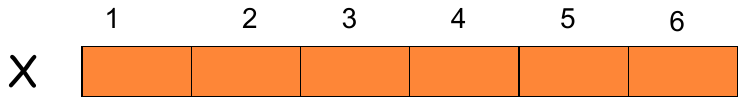
\includegraphics[scale=0.5]{./pictures/arreglo_unidimensional.png}
\end{figure}

\textbf{Índice o Subíndice:} designa la posición de un elemento en el arreglo.\\
\textbf{Operación \underline{Acceso}}. Se realiza a través del nombre del arreglo y entre corchetes el valor del índice.\\

Ejemplo:
\inputminted{./pseudocode.py:PseudocodeLexer -x}{./pseudocodigo/acceso.algo}

Las operaciones de \textbf{almacenamiento} se realizan usando el operador de
asignación y entregando un valor que será guardado en una posición del arreglo.\\

\inputminted{./pseudocode.py:PseudocodeLexer -x}{./pseudocodigo/asignacion.algo}

Cuando se usan arreglos se deben tomar los siguientes cuidados:

\begin{itemize}
  \item Dar valor inicial a los elementos del arreglo.
  \item Especificar siempre el valor del índice.
  \item Cuidar que los índices no tomen valores fuera de su rango.
\end{itemize}
\newpage

\subsection*{Arreglo de dos dimensiones (Matriz)}%
Está conformado por filas y columnas.

\begin{figure}[h!]
  \centering
  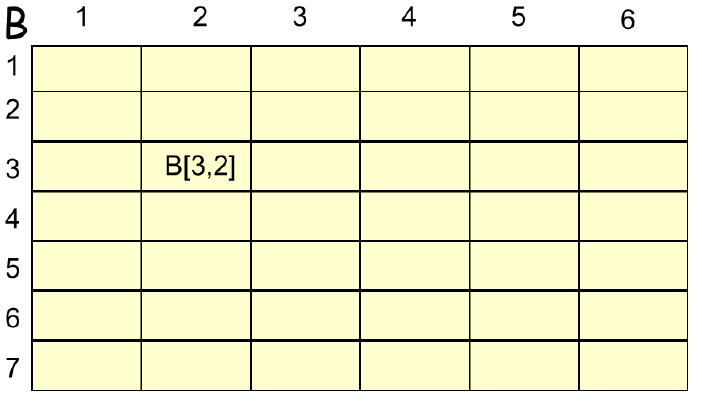
\includegraphics[scale=0.5]{./pictures/arreglo_bidimensional.png}
\end{figure}

\textbf{Operaccion de \underline{Acceso}}. Se realiza a través del nombre del
arreglo y entre corchetes el valor de los índices, considerando que el primero
indica el número de fila y el segundo el número de columna del elemento.\\

Ejemplo:
% pseudocodigo
\begin{minted}{./pseudocode.py:PseudocodeLexer -x}
    B[i,j]
\end{minted}

La operación de almacenamiento se realizan asignando un valor a una determinada posición del arreglo.\\

Es necesario tener la seguridad de que los valores usados para los índices sean
válidos, es decir que estén entre los valores limites definidos para el
arreglo.\\

\section*{Declaracion y referencia (Acceso)}%
\subsection*{Declaración}%
% pseudocodigo
\begin{minted}{./pseudocode.py:PseudocodeLexer -x}
    Tipo IdentificadorArreglo [tamano {, tamano}]
\end{minted}

\subsection*{Referencia a Arreglos}%
% pseudocodigo
\begin{minted}{./pseudocode.py:PseudocodeLexer -x}
    IdentificadorArreglo [Indice {, Indice}]
\end{minted}

Ejemplo (Unidimensional):
%pseudocodigo
\inputminted{./pseudocode.py:PseudocodeLexer -x}{./pseudocodigo/uso_unidimensional.algo}
\newpage

Ejemplo (Bidimensional):
%pseudocodigo
\inputminted{./pseudocode.py:PseudocodeLexer -x}{./pseudocodigo/uso_bidimensional.algo}

\subsection*{Vector}%
\subsubsection*{Ejemplo 1}%
Almacenar nota obtenida por cada uno de n alumnos (máximo 20) en el vector
notas. Mostrar cuantos alumnos aprobraron.\\
%pseudocodigo
\underline{\textit{Resolución en pseudocodigo}}\\
\inputminted{./pseudocode.py:PseudocodeLexer -x}{./pseudocodigo/001_ejemplo.algo}

%C++
\underline{\textit{Resolución en C++}}\\
\inputminted{cpp}{./cpp/001_ejemplo.cpp}


\subsubsection*{Ejercicio 1}%
Guardar 10 números en un arreglo. Mostrar cuántos valores son negativos, positivos y cero.\\

%pseudocodigo
\underline{\textit{Resolución en pseudocodigo}}\\
\inputminted{./pseudocode.py:PseudocodeLexer -x}{./pseudocodigo/001_ejercicio.algo}

%C++
\underline{\textit{Resolución en C++}}\\
\inputminted{cpp}{./cpp/001_ejercicio.cpp}


\section{Recordar que}%
En un arreglo.
\begin{itemize}
  \item Todos los datos serán del \textbf{mismo} tipo (homogéneo)
  \item La cantidad de elementos es \textbf{finita}.
  \item Para designar la posición de un elemento, se usa un valor entero llamado \textbf{índice}.
  \item Para referirse al arreglo, se usa un único \textbf{identificador}.
\end{itemize}
\newpage


\section*{Agradecimientos}
\textbf{Personas que apoyaron mandando psudocódigo y código en este documento:}\\

%---------------------------------------------------------------------------------
\vspace{3cm} 
\section*{¡Envianos tus soluciones!}
Si estás llevando este curso con los profesores Cabrera, Romero o Salinas;
envíanos tus soluciones en los diferentes lenguajes de programación que
conozcas al correo \href{mailto:gprunecode@gmail.com}{gprunecode@gmail.com}.
n.n \\ 

Las mejores soluciones tanto en el algoritmo como en el código, serán
publicadas en las siguientes ediciones de estos documentos.\\

El asunto del correo debe estar de la siguiente manera:\\
$NumeroDeSesion-Profesor-NumeroDeEjercicio$ \\
Por ejemplo:  \\
$01-Romero-01$ \\

Y dentro del correo adjuntar tu solución y nombre como quieras ser reconocido en caso de ser electo.

\vspace{2cm}
\LARGE\textit{RuneCode}


\end{document}

